\begin{frame} \frametitle{\vspace*{0.5cm}Results: Vorticity dynamics for the 10 MPa trapezoidal wave}
  \begin{figure}
    \centering
    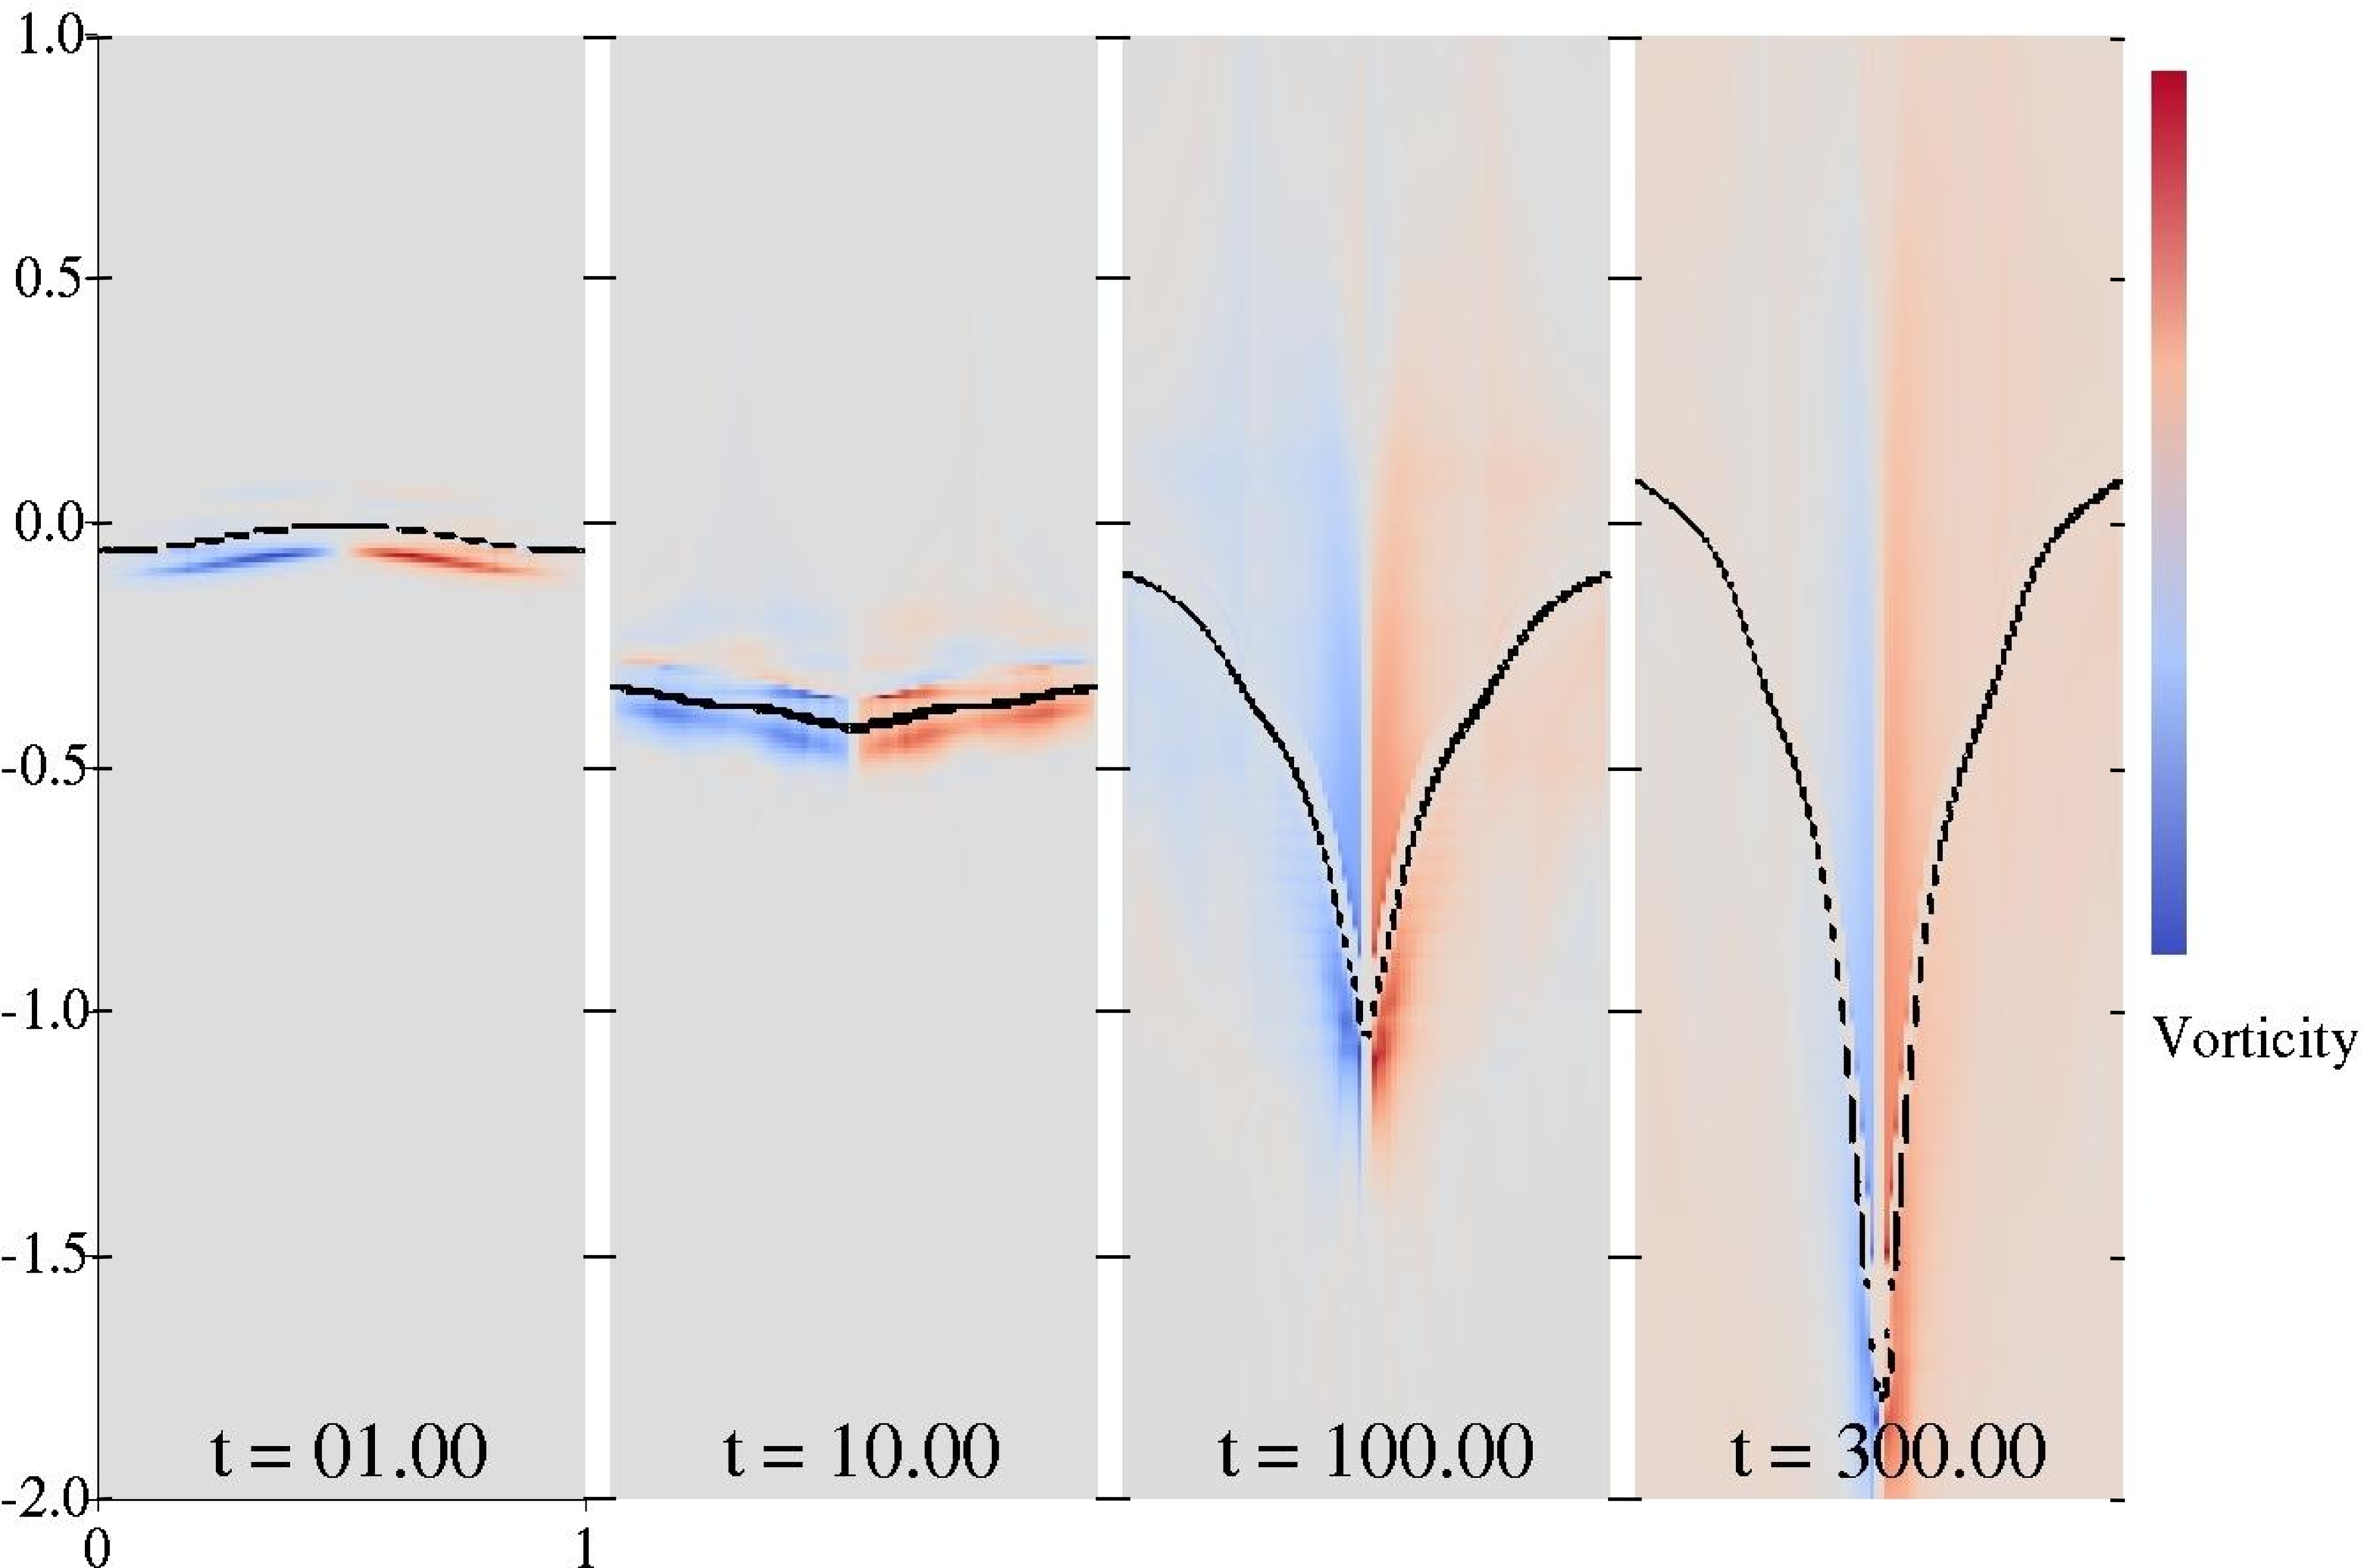
\includegraphics[width=0.8\textwidth]{../figs/lung_figs/snapshots_vorticity_t1}
  \end{figure}
  % 
  {\small
    \begin{itemize}
    \item Vorticity initially deposits in air-dominated $(y_0<0.5)$
      fluid of the interface.
    \item As the interface evolves, some vorticity advects with it.
    \end{itemize}
  }
  \note{
    {\small
      \begin{enumerate}
      \item So we look at the vorticity contours for the 10 MPa trapezoidal wave.
      \item Red indicates positive, counter clockwise vorticity, blue is negative, clockwise vorticity.
      \item A linear scale that changes each timestep is used for visual
        reasons.
      \item Black line indicates the 0.5 volume fraction line, where you have half water and air by volume.
      \item Air-domination is surprising to me because almost all of the wave
        is reflected so most of energy of the fluid stays in the water
        because of the high impedance mismatch. But we can explain this, and will later.
      \item At $t=1$, at the end of the compression, vorticity has been
        cleanly depositived in the interface, in predominately
        gas-dominated fluid.
      \item By the time the wave has passed, vorticity begins diffusing throughout the interface.
      \item As the interface evolves, much of the vorticity follows it, and some is left in its wake.
      \end{enumerate}
    }
  }
\end{frame}
%%% Local Variables:
%%% mode: latex
%%% TeX-master: "../main"
%%% End:
